%!TEX root = ../document.tex

\chapter{Einleitung}
\label{ch:intro}

\section{Über das Veranstaltungsverwaltungssystem INsite}
\label{sec:about_insite}

Seit dem Jahr 1999 pflegen Mitarbeiter der Stadt Ingolstadt und der \emph{Ingolstadt Tourismus und Kongress GmbH}\footnote{im Folgenden als \emph{ITK GmbH} bezeichnet} jährlich circa \numprint{4000} Veranstaltungen für den Internetauftritt der Stadt Ingolstadt.\footnote{siehe \url{http://www.ingolstadt.de}} Dies erfolgt bis dato mit dem webbasierten Veranstaltungsverwaltungssystem INsite\index{INsite}, welches von der \emph{response informationsdesign~gmbh~\&~co.~kg}\footnote{Schreibweise im Corporate Design, im Weiteren als \emph{response} aufgeführt} entwickelt wurde. Technische Grundlage für INsite stellt der Applicationserver Adobe\,ColdFusion\index{ColdFusion} sowie die zugehörige Programmiersprache CFML dar.

Veranstaltungen für INsite werden größtenteils händisch eingetragen. Zudem besteht für Bürger der Stadt die Möglichkeit, per Webformular\footnote{siehe\,\url{http://www2.ingolstadt.de/Aktuelles/Veranstaltungen/Veranstaltung_eintragen/}} Vorschläge für neue Veranstaltungen zu melden. Diese Eintragungen durchlaufen anschließend einen mehrstufigen Genehmigungsprozess -- welcher jedoch nicht in INsite abgebildet ist -- und werden dementsprechend entweder abgelehnt oder über INsite in den Kalender eingetragen.

Des Weiteren werden Sitzungen des Stadtrates automatisiert aus dem Ratsinformationssystem \emph{SessionNet} zu INsite synchronisiert.\footnote{vergleiche \url{http://www.ingolstadt.de/sessionnet/si0040.php}, SessionNet Veranstaltungskalender der Stadt Ingolstadt} Auch nach außen hin bietet INsite Schnittstellen an: Über einen SOAP"=Webservice werden aktuelle Veranstaltungen beispielsweise an den Webauftritt der ITK GmbH weitergegeben.

Allerdings fehlt es INsite an einigen, für Veranstaltungsverwaltungen typischen, Funktionen. So ist es beispielsweise nicht möglich, Serientermine zu erfassen. Auch der bereits erwähnte Genehmigungsprozess für bestimmte Veranstaltungen ist nicht in INsite integriert. Einen weiteren Mangel stellt das Design der Applikation dar, zu sehen in Abbildung \ref{fig:insite_screenshot_list}, welches als nicht mehr zeitgemäß betrachtet werden kann.

\begin{figure}[ht]
	\begin{margincap}
		\raggedright
		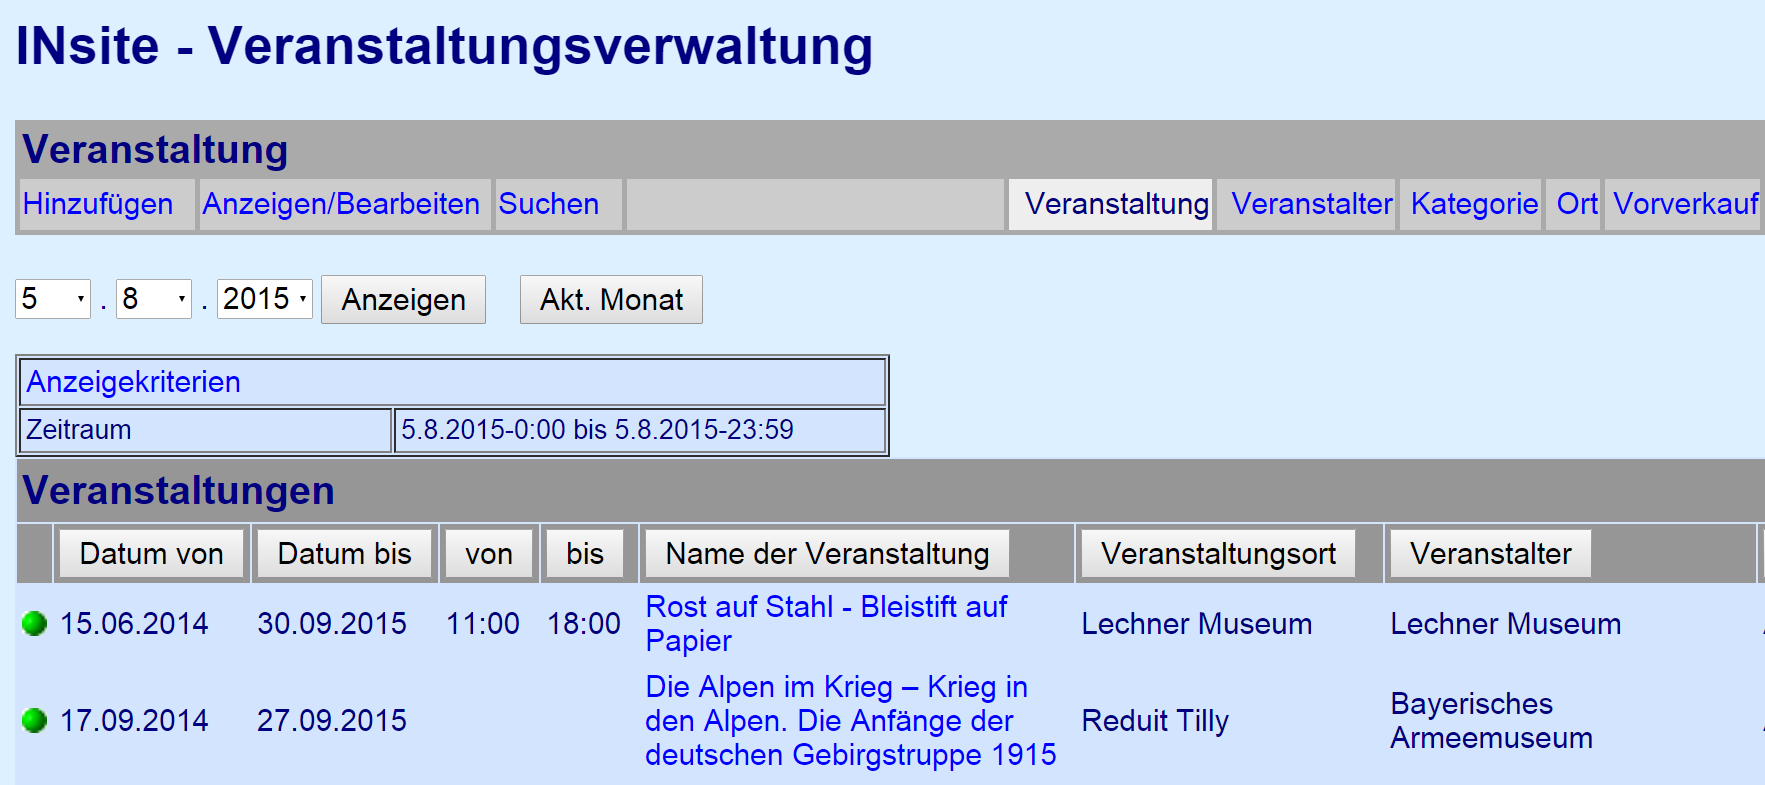
\includegraphics[width=0.98\defaultFigureWidth]{screenshot_insite_list.png}
		\caption[Screenshot von INsite]{Screenshot der aktuellen\footnote{Stand 05.08.2015} Version von INsite, angezeigt wird eine Liste von Veranstaltungen}
		\label{fig:insite_screenshot_list}
	\end{margincap}
\end{figure}

Aus diesen Gründen entschied sich die Stadtverwaltung der Stadt Ingolstadt für eine Neuentwicklung der Veranstaltungsverwaltung, welche bei response in Auftrag gegeben wurde. Auf dem \emph{ReEvent}\index{ReEvent} genannten Nachfolgesystem basiert wiederum die vorliegende Arbeit. Insbesondere die relevanten technischen Aspekte von ReEvent werden in Kapitel \ref{ch:reevent} dargestellt.


\section{Aufgabenstellung}
\label{sec:task}

Die von INsite\index{INsite} bereitgestellten Veranstaltungsdaten heutigen Datums werden in erster Linie auf der Startseite der städtischen Homepage angezeigt. Zudem existiert ein Formular zur gefilterten Anzeige aller vorliegenden Veranstaltungen, beispielsweise durch Eingrenzung des Zeitraums oder Festlegen einer Kategorie.\footnote{ siehe \url{http://www2.ingolstadt.de/Aktuelles/Veranstaltungen/}}
Ein optionales Suchfeld ergänzt die Filterfunktion. Wird ein Suchbegriff angegeben, so werden nur Veranstaltungen angezeigt, deren Namen oder Beschreibungstext die Zeichenfolge enthalten. Ein ähnliches Suchformular existiert im Backend von INsite. Serverseitig wird die Suche als parametrisierte SQL"=Abfrage realisiert.

\begin{figure}[ht]
	\begin{margincap}
		\raggedright
		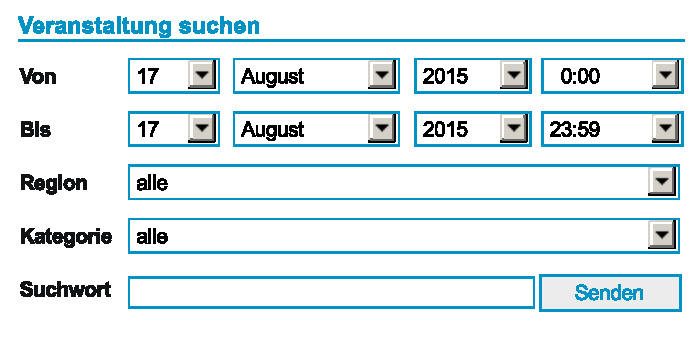
\includegraphics[width=\defaultFigureWidth]{screenshot_ingolstadt_filter_events.pdf}
		\caption[Screenshot des bestehenden Suchformulars]{Screenshot des bestehenden Formulars zur Filterung und Suche von Veranstaltungen im Frontend von INsite\footnote{Stand 17.08.2015}}
		\label{fig:insite_screenshot_filter_original}
	\end{margincap}
\end{figure}

Auch für ReEvent\index{ReEvent} wird eine Suchlösung benötigt. Neben der Minimallösung einer einfachen SQL-Abfrage existieren jedoch verschiedene Ansätze zur Suche, wie beispielsweise eine dedizierte SearchEngine\index{Search Engine} wie \emph{Apache Solr} \cite[S. 4]{Grainger.2014}. Gegenstand dieser Arbeit soll es sein, mögliche Suchsysteme zu recherchieren und in Hinblick auf die Tauglichkeit für die neue Veranstaltungsverwaltung ReEvent zu evaluieren. Die Ergebnisse der Evaluation sollen es erlauben, eine ausgewählte Suchlösung für die Suche in ReEvent zu empfehlen.


\section{Abgrenzung der Eigenleistung}
\label{sec:abgrenzung-der-eigenleistung}

Die Konzepte aus \ref{sec:ReEvent.Language.Nodes}, \ref{sec:content.objects}, \ref{sec:history.steps} und \ref{sec:workspaces} wurden von Mitarbeitern der response informationsdesign~gmbh~\&~co.~kg ausgearbeitet und werden an dieser Stelle lediglich als Hintergrundinformation wiedergegeben.
